
% THIS IS AN EXAMPLE DOCUMENT FOR VLDB 2012
% based on ACM SIGPROC-SP.TEX VERSION 2.7
% Modified by  Gerald Weber <gerald@cs.auckland.ac.nz>
% Removed the requirement to include *bbl file in here. (AhmetSacan, Sep2012)
% Fixed the equation on page 3 to prevent line overflow. (AhmetSacan, Sep2012)

\documentclass{vldb}
\usepackage{graphicx}
\usepackage{balance}  % for  \balance command ON LAST PAGE  (only there!)

% ****************** sungsoo's packages ****************************************
\usepackage{times}
%                              My Commands
\newcommand{\bi}{\begin{itemize}}
\newcommand{\ei}{\end{itemize}}
\newcommand{\be}{\begin{enumerate}}
\newcommand{\ee}{\end{enumerate}}
\newcommand{\ii}{\item}
\newtheorem{Def}{Definition}
\newtheorem{Lem}{Lemma}
\usepackage{algorithm}
\usepackage{algorithmicx}
\usepackage{algpseudocode}

\usepackage{graphicx}
\graphicspath{%
        {converted_graphics/}
        {./images/}
}
\usepackage{hyperref}
\usepackage{listings}
\usepackage{longtable}

% ****************** the following is needed for syntax highlighting
\usepackage{color}

\definecolor{dkgreen}{rgb}{0,0.6,0}
\definecolor{gray}{rgb}{0.5,0.5,0.5}
\definecolor{mauve}{rgb}{0.58,0,0.82}

\lstset{ %
  language=Java,                  % the language of the code
  basicstyle=\scriptsize,       % the size of the fonts that are used for the code
  numbers=left,                   % where to put the line-numbers
  numberstyle=\tiny\color{gray},  % the style that is used for the line-numbers
  stepnumber=1,                   % the step between two line-numbers. If it's 1, each line 
                                  % will be numbered
  numbersep=3.8pt,                  % how far the line-numbers are from the code
  backgroundcolor=\color{white},  % choose the background color. You must add \usepackage{color}
  showspaces=false,               % show spaces adding particular underscores
  showstringspaces=false,         % underline spaces within strings
  showtabs=false,                 % show tabs within strings adding particular underscores
  frame=false,                   % adds a frame around the code
  rulecolor=\color{black},        % if not set, the frame-color may be changed on line-breaks within not-black text (e.g. commens (green here))
  tabsize=2,                      % sets default tabsize to 2 spaces
  captionpos=b,                   % sets the caption-position to bottom
  breaklines=true,                % sets automatic line breaking
  breakatwhitespace=false,        % sets if automatic breaks should only happen at whitespace
  title=\lstname,                 % show the filename of files included with \lstinputlisting;
                                  % also try caption instead of title
  keywordstyle=\color{blue},          % keyword style
  commentstyle=\color{dkgreen},       % comment style
  stringstyle=\color{mauve},         % string literal style
  escapeinside={\%*}{*)},            % if you want to add a comment within your code
  morekeywords={*,...}               % if you want to add more keywords to the set
}
% ----------------
% General Packages
% ----------------

%\usepackage[margin = 1in]{geometry} % Margin of 1 inch each
\usepackage[usenames,dvipsnames]{xcolor} % Extended Color (Must be declared before tikz)

% Times font 
\usepackage{mathptmx}

% Necessity packages
%\usepackage{url, hyperref, amsmath, bm, listings, amssymb, multicol, framed, mdframed, mathabx}

% Language
\usepackage[english]{babel}

% Listing style
\usepackage{enumitem}

% Tikz
\usepackage{graphicx,  pgfplots, tikz, tkz-euclide, calc, datatool, datapie, databar} 
\usetkzobj{all} % For tikz-euclide
\usetikzlibrary{snakes}

% ----------------
% Paragraph Set up
% ----------------
%\usepackage{indentfirst}
%\setlength{\parskip}{6pt} 
%\setlength{\parindent}{20pt} 

% ----------------
% Listings Set up
% ----------------

\lstset{ %
language=SQL,                   % choose the language of the code
basicstyle=\ttfamily\small,
%basicstyle=\footnotesize,       % the size of the fonts that are used for the code
numbers=left,                   % where to put the line-numbers
numberstyle=\footnotesize,      % the size of the fonts that are used for the line-numbers
stepnumber=0,                   % the step between two line-numbers. If it is 1 each line will be numbered
numbersep=5pt,                  % how far the line-numbers are from the code
backgroundcolor=\color{white},  % choose the background color. You must add \usepackage{color}
commentstyle=\color{Aquamarine},
keywordstyle=\color{OrangeRed},
%basicstyle=\ttfamily\scriptsize,
showspaces=false,               % show spaces adding particular underscores
showstringspaces=false,         % underline spaces within strings
showtabs=false,                 % show tabs within strings adding particular underscores
%frame=single,           % adds a frame around the code
tabsize=2,          % sets default tabsize to 2 spaces
captionpos=b,           % sets the caption-position to bottom
breaklines=true,        % sets automatic line breaking
breakatwhitespace=false,    % sets if automatic breaks should only happen at whitespace
escapeinside={\%*}{*)},       % if you want to add a comment within your code
moredelim=**[is][\color{black}]{@}{@},
}

% ----------------
% New Commands
% ----------------

\newcommand{\encode}[1]{\left< #1 \right> }
\newcommand{\paren}[1]{\left( #1 \right) }
\newcommand{\setbrac}[1]{\left\{ #1 \right\} }
\newcommand{\brac}[1]{\left[ #1 \right]}

\newcommand{\ands}{\wedge}
\newcommand{\ors}{\vee}
\newcommand{\thens}{\to}
\newcommand{\iffs}{\leftrightarrow}
\newcommand{\nots}{\sim}
\newcommand{\fd}{\rightarrow}
\newcommand{\mvd}{\twoheadrightarrow}
\newcommand{\inter}{\cap}
\newcommand{\union}{\cup}
\newcommand{\select}{\sigma}
\newcommand{\diff}{-}
\newcommand{\project}{\pi}
\newcommand{\rename}{\rho}
\newcommand{\join}{\Join}
\newcommand{\Null}{\text{NULL}}

%-------------------------------------
% CS61 students begin copying here
%\usepackage{amssymb}
%
%\def\ojoin{\setbox0=\hbox{$\bowtie$}%
%  \rule[-.02ex]{.25em}{.4pt}\llap{\rule[\ht0]{.25em}{.4pt}}}
%\def\leftouterjoin{\mathbin{\ojoin\mkern-5.8mu\bowtie}}
%\def\rightouterjoin{\mathbin{\bowtie\mkern-5.8mu\ojoin}}
%\def\fullouterjoin{\mathbin{\ojoin\mkern-5.8mu\bowtie\mkern-5.8mu\ojoin}}
%
% Relational algebra symbols from ftp://reports.stanford.edu/www/dbgroup_only/latex-macros.html
%\newcommand{\select}{\mbox{\Large$\sigma$}}
%\newcommand{\cross}{\mbox{$\times$}}
%\newcommand{\intersection}{\mbox{$\cap$}}
%\newcommand{\intersect}{\mbox{$\cap$}}
%\newcommand{\union}{\mbox{$\cup$}}
%\newcommand{\join}{\mbox{$\Join$}}
%\newcommand{\leftsemijoin}{\mbox{$\mathrel{\raise1pt\hbox{\vrule height5pt
%depth0pt width0.6pt\hskip-1.5pt$>$\hskip -2.5pt$<$}}$}}
%\newcommand{\rightsemijoin}{\mbox{$\mathrel{\raise1pt\hbox{\hskip-1.5pt$>$\hskip -2.5pt$<$\hskip -1.1pt\vrule height5pt
%depth0pt width0.6pt}}$}}
%\newcommand{\project}{\mbox{\Large$\pi$}}
%\newcommand{\Project}{\mbox{$\Pi$}}
%\newcommand{\aggregatefn}{\mbox{\Large$G$}}
%
% CS61 students end copying here
%-------------------------------------

% ****************** end of sungsoo's packages ****************************************


\begin{document}

% ****************** TITLE ****************************************

%\title{A Sample {\ttlit Proceedings of the VLDB Endowment} Paper in LaTeX
%Format\titlenote{for use with vldb.cls}}

\title{Query Processing}

% possible, but not really needed or used for PVLDB:
%\subtitle{[Extended Abstract]
%\titlenote{A full version of this paper is available as\textit{Author's Guide to Preparing ACM SIG Proceedings Using \LaTeX$2_\epsilon$\ and BibTeX} at \texttt{www.acm.org/eaddress.htm}}}

% ****************** AUTHORS **************************************

% You need the command \numberofauthors to handle the 'placement
% and alignment' of the authors beneath the title.
%
% For aesthetic reasons, we recommend 'three authors at a time'
% i.e. three 'name/affiliation blocks' be placed beneath the title.
%
% NOTE: You are NOT restricted in how many 'rows' of
% "name/affiliations" may appear. We just ask that you restrict
% the number of 'columns' to three.
%
% Because of the available 'opening page real-estate'
% we ask you to refrain from putting more than six authors
% (two rows with three columns) beneath the article title.
% More than six makes the first-page appear very cluttered indeed.
%
% Use the \alignauthor commands to handle the names
% and affiliations for an 'aesthetic maximum' of six authors.
% Add names, affiliations, addresses for
% the seventh etc. author(s) as the argument for the
% \additionalauthors command.
% These 'additional authors' will be output/set for you
% without further effort on your part as the last section in
% the body of your article BEFORE References or any Appendices.

\numberofauthors{1} %  in this sample file, there are a *total*
% of EIGHT authors. SIX appear on the 'first-page' (for formatting
% reasons) and the remaining two appear in the \additionalauthors section.

\author{
% You can go ahead and credit any number of authors here,
% e.g. one 'row of three' or two rows (consisting of one row of three
% and a second row of one, two or three).
%
% The command \alignauthor (no curly braces needed) should
% precede each author name, affiliation/snail-mail address and
% e-mail address. Additionally, tag each line of
% affiliation/address with \affaddr, and tag the
% e-mail address with \email.
%
% 1st. author
\alignauthor
Sung-Soo Kim\\ %\titlenote{Dr.~Trovato insisted his name be first.}\\
       \affaddr{Data Management Research Section}\\
       \affaddr{Electronics and Telecommunications Research Institute}\\
       \affaddr{128 Gajeong-ro, Yuseong-gu}\\
       \affaddr{Daejeon, South Korea}\\
       \email{\normalsize \it sungsoo@etri.re.kr}
% 2nd. author
%\alignauthor
%G.K.M. Tobin\titlenote{The secretary disavows
%any knowledge of this author's actions.}\\
%       \affaddr{Institute for Clarity in Documentation}\\
%       \affaddr{P.O. Box 1212}\\
%       \affaddr{Dublin, Ohio 43017-6221}\\
%       \email{webmaster@marysville-ohio.com}
% 3rd. author
%\alignauthor Lars Th{\Large{\sf{\o}}}rv{$\ddot{\mbox{a}}$}ld\titlenote{This author is the
%one who did all the really hard work.}\\
%       \affaddr{The Th{\large{\sf{\o}}}rv{$\ddot{\mbox{a}}$}ld Group}\\
%       \affaddr{1 Th{\large{\sf{\o}}}rv{$\ddot{\mbox{a}}$}ld Circle}\\
%       \affaddr{Hekla, Iceland}\\
%       \email{larst@affiliation.org}
%\and  % use '\and' if you need 'another row' of author names
% 4th. author
%\alignauthor Lawrence P. Leipuner\\
%       \affaddr{Brookhaven Laboratories}\\
%       \affaddr{Brookhaven National Lab}\\
%       \affaddr{P.O. Box 5000}\\
%       \email{lleipuner@researchlabs.org}
% 5th. author
%\alignauthor Sean Fogarty\\
%       \affaddr{NASA Ames Research Center}\\
%       \affaddr{Moffett Field}\\
%       \affaddr{California 94035}\\
%       \email{fogartys@amesres.org}
% 6th. author
%\alignauthor Charles Palmer\\
%       \affaddr{Palmer Research Laboratories}\\
%       \affaddr{8600 Datapoint Drive}\\
%       \affaddr{San Antonio, Texas 78229}\\
%       \email{cpalmer@prl.com}
}
% There's nothing stopping you putting the seventh, eighth, etc.
% author on the opening page (as the 'third row') but we ask,
% for aesthetic reasons that you place these 'additional authors'
% in the \additional authors block, viz.
%\additionalauthors{Additional authors: John Smith (The Th{\o}rv\"{a}ld Group, {\texttt{jsmith@affiliation.org}}), Julius P.~Kumquat
%(The \raggedright{Kumquat} Consortium, {\small \texttt{jpkumquat@consortium.net}}), and Ahmet Sacan (Drexel University, {\small \texttt{ahmetdevel@gmail.com}})}
%\date{30 July 1999}
% Just remember to make sure that the TOTAL number of authors
% is the number that will appear on the first page PLUS the
% number that will appear in the \additionalauthors section.


\maketitle

\begin{abstract}
In this technical report, we describe the overview of query processing  in the distributed database systems. 

The success of relational database technology in data processing is due, in part, to the availability of non-procedural languages (i.e., SQL), which can significantly improve application development and end-user productivity. By hiding the low-level details about the physical organization of the data, relational database languages allow the expression of complex queries in a concise and simple fashion. In particular, to construct the answer to the query, the user does not precisely specify the procedure to follow. This procedure is actually devised by a DBMS module, usually called a \textit{query processor}. This relieves the user from query optimization, a time-consuming task that is best handled by the query processor, since it can exploit a large amount of useful information about the data.

Because it is a critical performance issue, query processing has received (and continues to receive) considerable attention in the context of both centralized and distributed DBMSs. However, the query processing problem is much more difficult in distributed environments than in centralized ones, because a larger number of parameters affect the performance of distributed queries. In particular, the relations involved in a distributed query may be fragmented and/or replicated, thereby inducing communication overhead costs. Furthermore, with many sites to access, query response time may become very high.

We give an overview of query processing in distributed DBMSs, leaving the details of the important aspects of distributed query processing. 
\end{abstract}


\section{Introduction}

\textit{Query processing} refers to the range of activities involved in extracting data from a database. The activities include translation of queries in high-level database languages into expressions that can be used at the physical level of the file system, a variety of query-optimizing transformations, and actual evaluation of queries.

The aims of query processing are to transform a query written in a high-level language, typically SQL, into a correct and efficient execution strategy expressed in a low-level language (implementing the relational algebra), and to execute the strategy to retrieve the required data.

The steps involved in processing a query appear in Figure ref{fig:steps}. The basic steps
are:

\be
\ii Parsing and translation.
\ii Optimization.
\ii Evaluation.
\ee

Before query processing can begin, the system must translate the query into
a usable form. A language such as SQL is suitable for human use, but is ill suited
to be the system’s internal representation of a query. A more useful internal
representation is one based on the extended relational algebra.

\begin{figure}[htb]
\centering
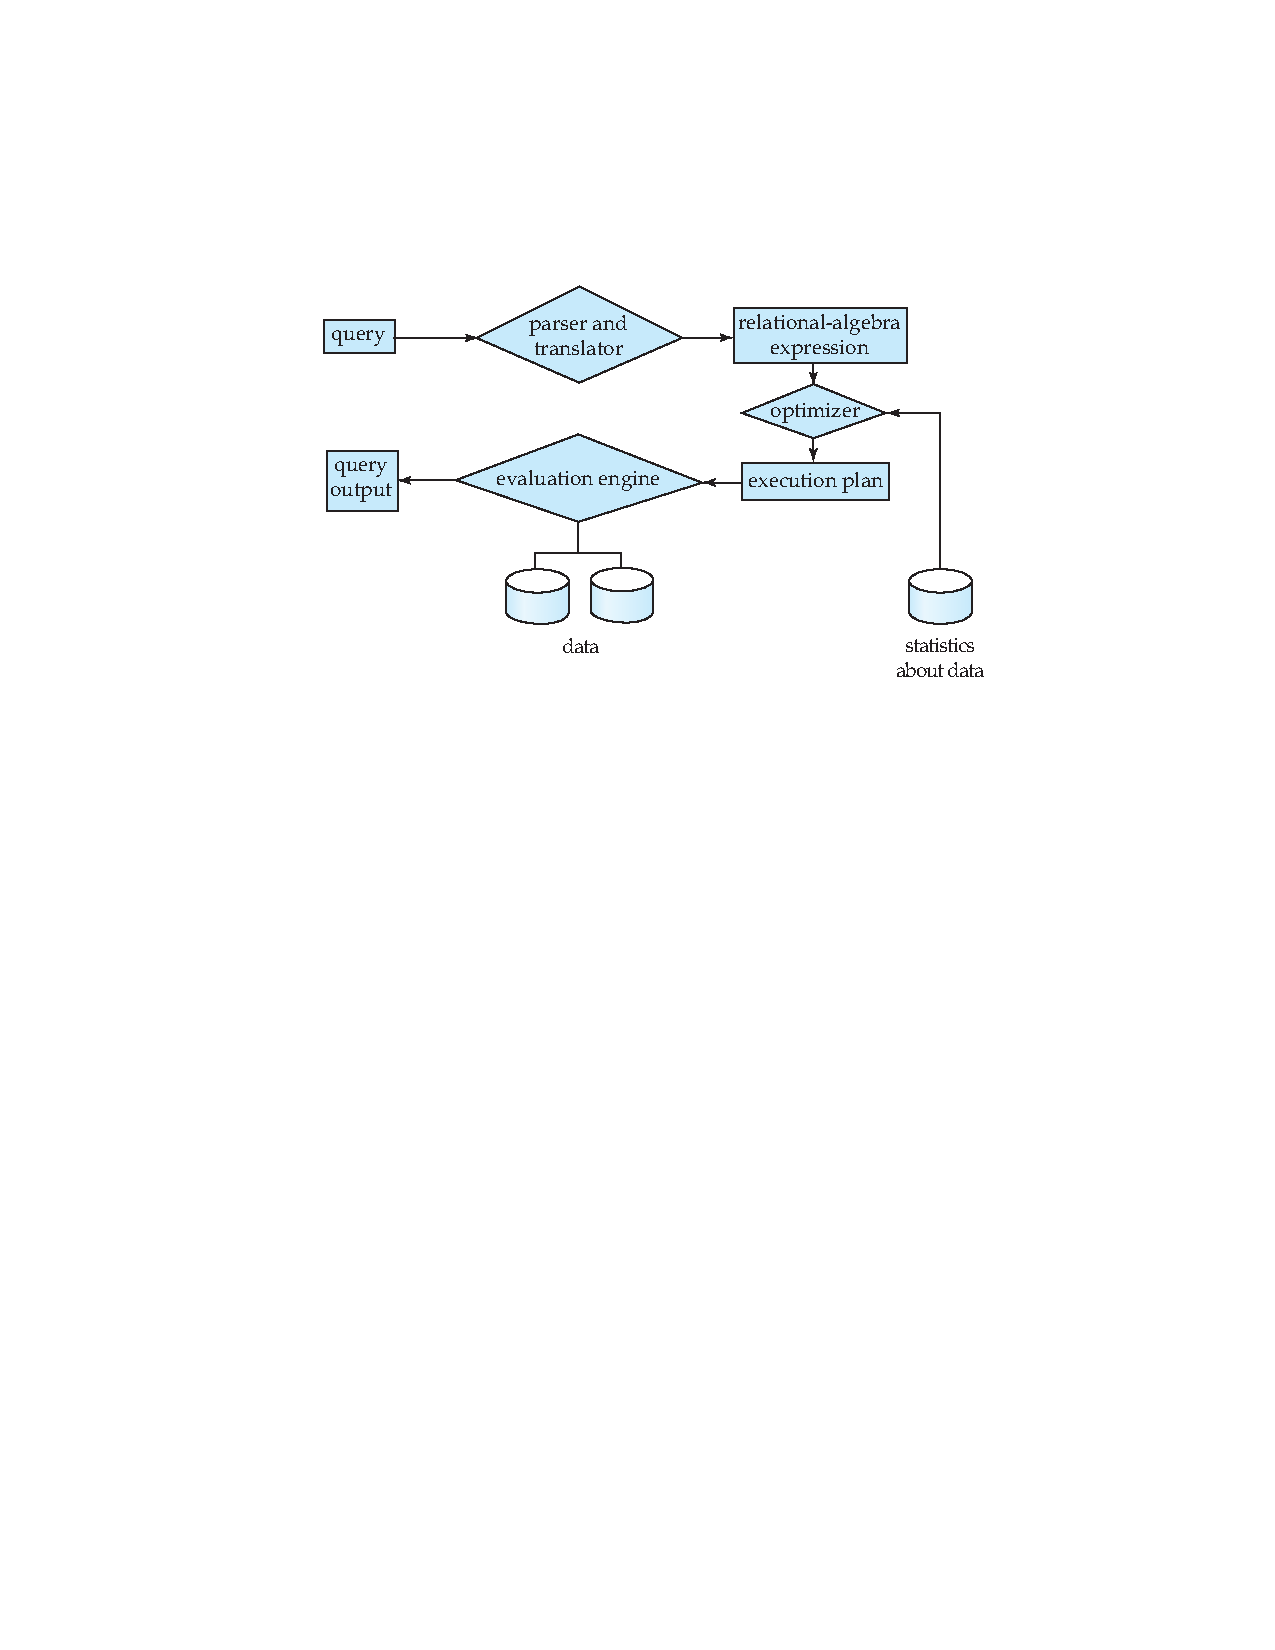
\includegraphics[width=0.48\textwidth]{query-processing-steps}
\caption{Steps in query processing.}
\label{fig:steps}
\end{figure}

Thus, the first action the system must take in query processing is to translate
a given query into its internal form.This translation process is similar to the work
performed by the parser of a compiler. In generating the internal form of the
query, the parser checks the syntax of the user’s query, verifies that the relation
names appearing in the query are names of the relations in the database, and
so on. The system constructs a parse-tree representation of the query, which it
then translates into a relational-algebra expression. If the query was expressed
in terms of a view, the translation phase also replaces all uses of the view by the
relational-algebra expression that defines the view. 
For materialized views, the expression defining the view has already been evaluated and stored. 
Therefore, the stored relation can be used, instead of uses of the view being replaced by the expression defining the view
Most compiler texts cover
parsing in detail.



Given a query, there are generally a variety of methods for computing the
answer. For example, we have seen that, in SQL, a query could be expressed in
several different ways. Each SQL query can itself be translated into a relational algebra
expression in one of several ways. Furthermore, the relational-algebra
representation of a query specifies only partially how to evaluate a query; there are
usually several ways to evaluate relational-algebra expressions. As an illustration,
consider the query:

\begin{lstlisting}
		SELECT salary
		FROM instructor
		WHERE salary < 75000;
\end{lstlisting}
This query can be translated into either of the following relational-algebra expressions:
\bi
\ii $\select_{salary<75000}(\project_{salary}(instructor))$
\ii $\project_{salary}(\select_{salary<75000}(instructor))$
\ei

Further, we can execute each relational-algebra operation by one of several different algorithms. For example, to implement the preceding selection, we can search every tuple in instructor to find tuples with salary less than 75000. If a B+-tree index is available on the attribute salary, we can use the index instead to locate the tuples.

 To specify fully how to evaluate a query, we need not only to provide the relational-algebra expression, but also to annotate it with instructions specifying how to evaluate each operation. 
Annotations may state the algorithm to be used for a specific operation, or the particular index or indices to use. A relational algebra
operation annotated with instructions on how to evaluate it is called an \textit{evaluation primitive}. 
A sequence of primitive operations that can be used to evaluate a query is a \textit{query-execution plan} or \textit{query-evaluation plan}. 
Figure \ref{fig:query} illustrates an evaluation plan for our example query, in which a particular index
(denoted in the figure as “index 1”) is specified for the selection operation. The
\textit{query-execution engine} takes a query-evaluation plan, executes that plan, and
returns the answers to the query.

\begin{figure}[htb]
\centering
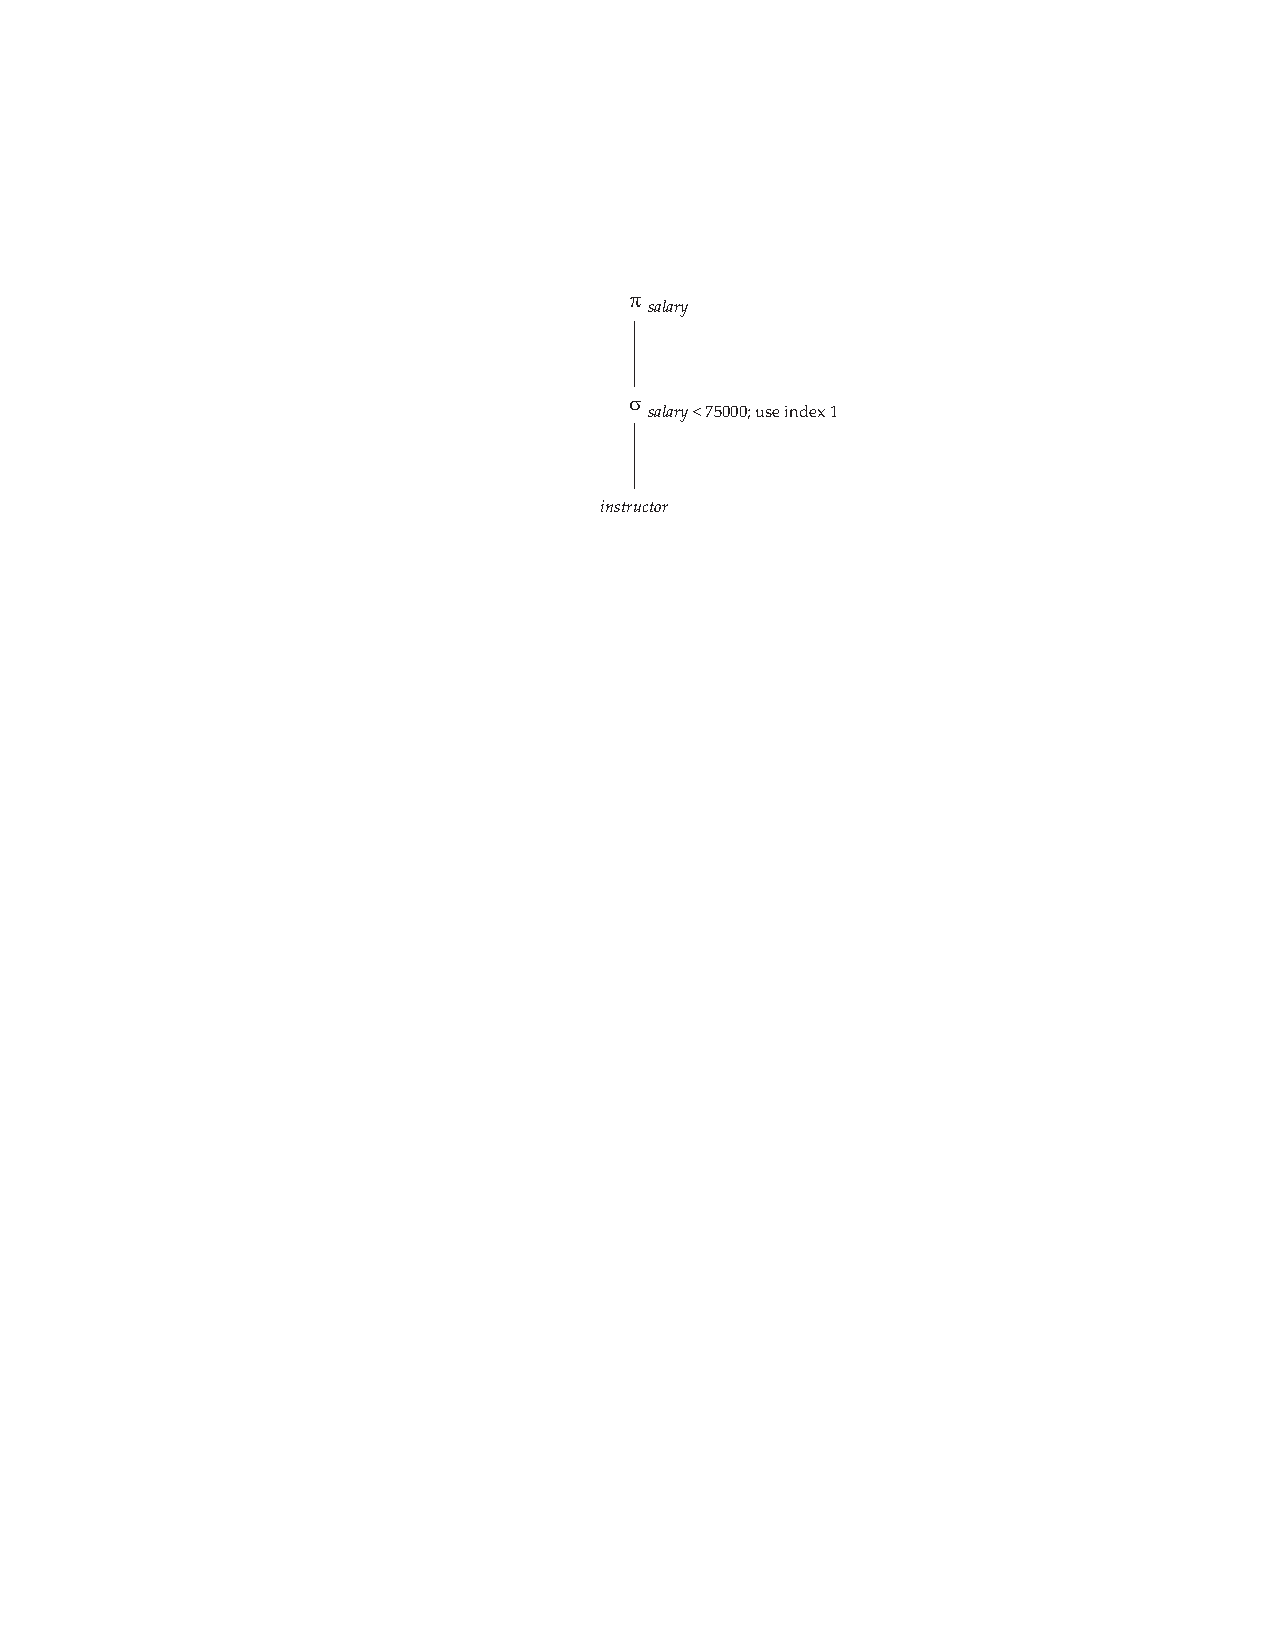
\includegraphics[width=0.25\textwidth]{query}
\caption{A query-evaluation plan.}
\label{fig:query}
\end{figure}

The different evaluation plans for a given query can have different costs. 
We do not expect users to write their queries in a way that suggests the most efficient evaluation plan. 
Rather, it is the responsibility of the system to construct a query evaluation plan that minimizes the cost of query evaluation; this task is called
\textit{query optimization}.

Once the query plan is chosen, the query is evaluated with that plan, and the result of the query is output.
The sequence of steps already described for processing a query is representative;
not all databases exactly follow those steps. For instance, instead of using the relational-algebra representation, several databases use an annotated parse tree representation based on the structure of the given SQL query. 
However, the concepts that we describe here form the basis of query processing in databases.
In order to optimize a query, a query optimizer must know the cost of each operation. 
Although the exact cost is hard to compute, since it depends on many parameters such as actual memory available to the operation, it is possible to get a rough estimate of execution cost for each operation.

\section{Measures of Query Cost}

There are multiple possible evaluation plans for a query, and it is important to be able to compare the alternatives in terms of their (estimated) cost, and choose
the best plan. 
To do so, we must estimate the cost of individual operations, and combine them to get the cost of a query evaluation plan. 
%Thus, as we study evaluation algorithms for each operation later in this chapter, we also outline how to estimate the cost of the operation.
The cost of query evaluation can be measured in terms of a number of different resources, including disk accesses, CPU time to execute a query, and, in
a distributed or parallel database system, the cost of communication.

In large database systems, the cost to access data from disk is usually the most important cost, since disk accesses are slow compared to in-memory operations.
Moreover, CPU speeds have been improving much faster than have disk speeds.
Thus, it is likely that the time spent in disk activity will continue to dominate the total time to execute a query. 
The CPU time taken for a task is harder to estimate since it depends on low-level details of the execution code. 
Although real-life query optimizers do take CPU costs into account, for simplicity in this article we ignore CPU costs and use only disk-access costs to measure the cost of a query-evaluation plan.
We use the \textit{number of block transfers} from disk and the \textit{number of disk seeks} to estimate the cost of a query-evaluation plan. 
If the disk subsystem takes an average of $t_T$ seconds to transfer a block of data, and has an average block-access time (disk seek time plus rotational latency) of $t_S$ seconds, then an operation that transfers $b$ blocks and performs $S$ seeks would take $b ∗ t_T + S ∗ t_S$ seconds. 
The values of $t_T$ and $t_S$ must be calibrated for the disk system used, but typical values for high-end disks today would be $t_S = 4$ milliseconds and $t_T = 0.1$ milliseconds, assuming a 4-kilobyte block size and a transfer rate of 40 megabytes per second.

We can refine our cost estimates further by distinguishing block reads from block writes, since block writes are typically about twice as expensive as reads
(this is because disk systems read sectors back after they are written to verify that the write was successful). 
For simplicity, we ignore this detail, and leave it to you to work out more precise cost estimates for various operations.

The cost estimates we give do not include the cost of writing the final result of an operation back to disk. 
These are taken into account separately where required.
The costs of all the algorithms that we consider depend on the size of the buffer in main memory. 
In the best case, all data can be read into the buffers, and the disk does not need to be accessed again. 
In the worst case, we assume that the buffer can hold only a few blocks of data—approximately one block per relation.
When presenting cost estimates, we generally assume the worst case.


In addition, although we assume that data must be read from disk initially, it is possible that a block that is accessed is already present in the in-memory buffer.
Again, for simplicity, we ignore this effect; as a result, the actual disk-access cost during the execution of a plan may be less than the estimated cost.

The \textit{response time} for a query-evaluation plan (that is, the wall-clock time required to execute the plan), assuming no other activity is going on in the
computer, would account for all these costs, and could be used as a measure of the cost of the plan. Unfortunately, the response time of a plan is very hard to
estimate without actually executing the plan, for the following reasons:

\be
\ii The response time depends on the contents of the buffer when the query
begins execution; this information is not available when the query is optimized,
and is hard to account for even if it were available.
\ii In a system with multiple disks, the response time depends on how accesses
are distributed among disks, which is hard to estimate without detailed
knowledge of data layout on disk.
\ee

Interestingly, a plan may get a better response time at the cost of extra resource
consumption. For example, if a system has multiple disks, a plan $A$ that requires
extra disk reads, but performs the reads in parallel across multiple disks may
finish faster than another plan $B$ that has fewer disk reads, but from only one
disk. However, if many instances of a query using plan A run concurrently, the
overall response time may actually be more than if the same instances are executed
using plan $B$, since plan $A$ generates more load on the disks.

As a result, instead of trying to minimize the response time, optimizers generally
try to minimize the total \textit{resource consumption} of a query plan. Our model
of estimating the total disk access time (including seek and data transfer) is an
example of such a resource consumption–based model of query cost.

\section{Selection Operation}

In query processing, the \textbf{file scan} is the lowest-level operator to access data. 
File scans are search algorithms that locate and retrieve records that fulfill a selection condition. 
In relational systems, a file scan allows an entire relation to be read in those cases where the relation is stored in a single, dedicated file.

\subsection{Cost Estimates for Selection Algorithms}
Cost estimates are shown in Figure \ref{fig:cost}. For more details, please refer to the reference books.

\begin{figure}[htb]
\centering
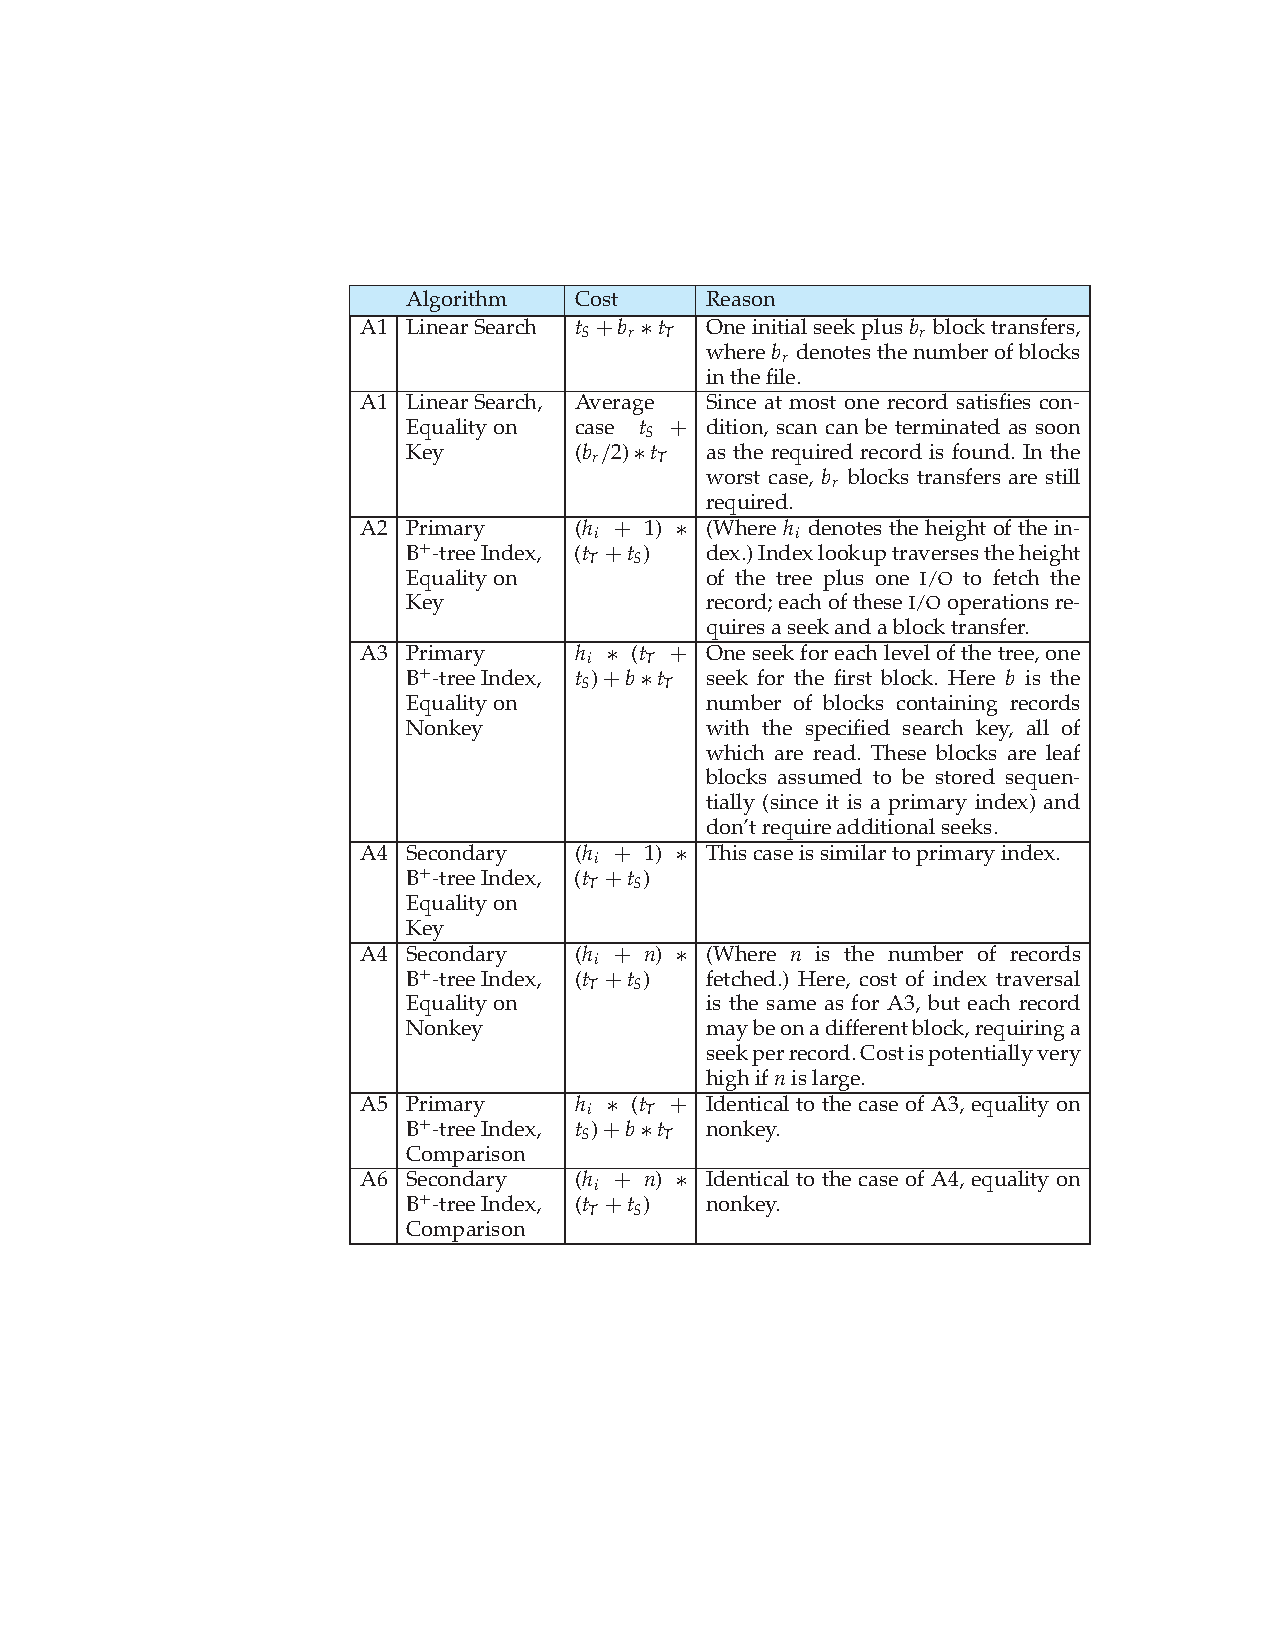
\includegraphics[width=0.48\textwidth]{selection_algorithms}
\caption{Cost estimates for selection algorithms.}
\label{fig:cost}
\end{figure}

Consider a selection operation on a relation whose tuples are stored together in one file. 
The most straightforward way of performing a selection is as follows:
\bi
\ii \textbf{A1 (linear search).} In a linear search, the system scans each file block and
tests all records to see whether they satisfy the selection condition. An initial
seek is required to access the first block of the file. In case blocks of the file
are not stored contiguously, extra seeks may be required, but we ignore this
effect for simplicity.

Although it may be slower than other algorithms for implementing selection,
the linear-search algorithm can be applied to any file, regardless of the
ordering of the file, or the availability of indices, or the nature of the selection
operation. The other algorithms that we shall study are not applicable in all
cases, but when applicable they are generally faster than linear search.
\ei

Cost estimates for linear scan, as well as for other selection algorithms, are
shown in Figure \ref{fig:cost}. In the figure, we use $h_i$ to represent the height of the B+-
tree. Real-life optimizers usually assume that the root of the tree is present in the
in-memory buffer since it is frequently accessed. Some optimizers even assume
that all but the leaf level of the tree is present in memory, since they are accessed
relatively frequently, and usually less than 1 percent of the nodes of a B+-tree are
nonleaf nodes. The cost formulae can be modified appropriately.

Index structures are referred to as \textbf{access paths}, since they provide a path
through which data can be located and accessed. We pointed out
that it is efficient to read the records of a file in an order corresponding closely to
physical order. Recall that a \textit{primary index} (also referred to as a \textit{clustering index}) is
an index that allows the records of a file to be read in an order that corresponds
to the physical order in the file. An index that is not a primary index is called a
\textit{secondary index}.

Search algorithms that use an index are referred to as \textbf{index scans}. We use the
selection predicate to guide us in the choice of the index to use in processing the
query. Search algorithms that use an index are:

\bi
\ii \textbf{A2 (primary index, equality on key).} For an equality comparison on a key
attribute with a primary index,we can use the index to retrieve a single record
that satisfies the corresponding equality condition. Cost estimates are shown
in Figure \ref{fig:cost}.
\ii \textbf{A3 (primary index, equality on nonkey).} We can retrieve multiple records
by using a primary index when the selection condition specifies an equality
comparison on a nonkey attribute, A. The only difference from the previous
case is that multiple records may need to be fetched. However, the records
must be stored consecutively in the file since the file is sorted on the search
key. Cost estimates are shown in Figure \ref{fig:cost}.
\ii \textbf{A4 (secondary index, equality).} Selections specifying an equality condition
can use a secondary index. This strategy can retrieve a single record if the
equality condition is on a key;multiple records may be retrieved if the indexing
field is not a key.

In the first case, only one record is retrieved. The time cost in this case is
the same as that for a primary index (case A2).

In the second case, each record may be resident on a different block, which
may result in one I/O operation per retrieved record,with each I/O operation
requiring a seek and a block transfer. The worst-case time cost in this case is
$(h_i + n) ∗ (t_S + t_T )$, where n is the number of records fetched, if each record
is in a different disk block, and the block fetches are randomly ordered. The
worst-case cost could become even worse than that of linear search if a large
number of records are retrieved.

If the in-memory buffer is large, the block containing the record may
already be in the buffer. It is possible to construct an estimate of the average
or expected cost of the selection by taking into account the probability of the
block containing the record already being in the buffer. For large buffers, that
estimate will be much less than the worst-case estimate.
\ei

In certain algorithms, including A2, the use of a B+-tree file organization can
save one access since records are stored at the leaf-level of the tree.
When records are stored in a B+-tree file organization
or other file organizations that may require relocation of records, secondary
indices usually do not store pointers to the records. Instead, secondary indices
store the values of the attributes used as the search key in a B+-tree file organization.
Accessing a record through such a secondary index is then more expensive:
First the secondary index is searched to find the primary index search-key values,
then the primary index is looked up to find the records. The cost formulae
described for secondary indices have to be modified appropriately if such indices
are used.

\subsection{Selections Involving Comparisons}
Consider a selection of the form !A≤v(r). We can implement the selection either
by using linear search or by using indices in one of the following ways:
\bi
\ii \textbf{A5 (primary index, comparison).} A primary ordered index (for example, a
primary B+-tree index) can be used when the selection condition is a comparison.
For comparison conditions of the form $A > v$ or $A \geq v$, a primary
index on A can be used to direct the retrieval of tuples, as follows: For $A \geq v$,
we look up the value v in the index to find the first tuple in the file that has
a value of $A = v$. A file scan starting from that tuple up to the end of the file
returns all tuples that satisfy the condition. For A> v, the file scan starts with
the first tuple such that $A > v$. The cost estimate for this case is identical to
that for case A3.

For comparisons of the form $A < v$ or $A \leq v$, an index lookup is not
required. For $A< v$, we use a simple file scan starting fromthe beginning of
the file, and continuing up to (but not including) the first tuple with attribute
$A = v$. The case of $A \leq v$ is similar, except that the scan continues up to (but
not including) the first tuple with attribute $A> v$. In either case, the index is
not useful.
\ii \textbf{A6 (secondary index, comparison).} We can use a secondary ordered index
to guide retrieval for comparison conditions involving $<, \leq, \geq$, or $>$. The
lowest-level index blocks are scanned, either from the smallest value up to $v$
(for $<$ and $\leq$), or from v up to the maximum value (for $>$ and $\geq$).

The secondary index provides pointers to the records, but to get the actual
records we have to fetch the records by using the pointers. This step may
require an I/O operation for each record fetched, since consecutive records
may be on different disk blocks; as before, each I/O operation requires a disk
seek and a block transfer. If the number of retrieved records is large, using
the secondary index may be even more expensive than using linear search.
Therefore the secondary index should be used only if very few records are
selected.
\ei

\subsection{Implementation of Complex Selections}
So far, we have considered only simple selection conditions of the form A op B,
where op is an equality or comparison operation.We now consider more complex
selection predicates.
\bi
\ii \textbf{Conjunction:} A \textit{conjunctive selection} is a selection of the form:
$$\select_{\theta_1 \ands \theta_2 \ands \cdots \ands \theta_n} (r)$$
\ii \textbf{Disjunction:} A \textit{disjunctive selection} is a selection of the form:
$$\select_{\theta_1 \ors \theta_2 \ors \cdots \ors \theta_n} (r)$$
\ei

A disjunctive condition is satisfied by the union of all records satisfying the
individual, simple conditions $\theta_i$ .
\bi
\ii \textbf{Negation:} The result of a selection $\select_{\neg \theta} (r)$ is the set of tuples of $r$ for which
the condition $\theta$ evaluates to false. In the absence of nulls, this set is simply
the set of tuples in r that are not in $\select_{\theta} (r)$.
\ei

We can implement a selection operation involving either a conjunction or a
disjunction of simple conditions by using one of the following algorithms:
\bi
\ii \textbf{A7 (conjunctive selection using one index). } We first determine whether an
access path is available for an attribute in one of the simple conditions. If
one is, one of the selection algorithms A2 through A6 can retrieve records
satisfying that condition.We complete the operation by testing, in thememory
buffer, whether or not each retrieved record satisfies the remaining simple
conditions.

To reduce the cost, we choose a $\theta_i$ and one of algorithms A1 through A6 for
which the combination results in the least cost for $\select_{\theta_i}(r)$. The cost of algorithm
A7 is given by the cost of the chosen algorithm.
\ii \textbf{A8 (conjunctive selection using composite index).} An appropriate \textit{composite
index} (that is, an index on multiple attributes) may be available for some
conjunctive selections. If the selection specifies an equality condition on two
or more attributes, and a composite index exists on these combined attribute
fields, then the index can be searched directly. The type of index determines
which of algorithms A2, A3, or A4 will be used.
\ii \textbf{A9 (conjunctive selection by intersection of identifiers).} Another alternative
for implementing conjunctive selection operations involves the use of
record pointers or record identifiers. This algorithm requires indices with
record pointers, on the fields involved in the individual conditions. The algorithm
scans each index for pointers to tuples that satisfy an individual
condition. The intersection of all the retrieved pointers is the set of pointers
to tuples that satisfy the conjunctive condition. The algorithm then uses the
pointers to retrieve the actual records. If indices are not available on all the
individual conditions, then the algorithm tests the retrieved records against
the remaining conditions.

The cost of algorithm A9 is the sum of the costs of the individual index scans,
plus the cost of retrieving the records in the intersection of the retrieved lists of
pointers. This cost can be reduced by sorting the list of pointers and retrieving
records in the sorted order. Thereby, (1) all pointers to records in a block come
together, hence all selected records in the block can be retrieved using a single
I/O operation, and (2) blocks are read in sorted order, minimizing disk-arm
movement.
\ii \textbf{A10 (disjunctive selection by union of identifiers).}  If access paths are available
on all the conditions of a disjunctive selection, each index is scanned
for pointers to tuples that satisfy the individual condition. The union of all
the retrieved pointers yields the set of pointers to all tuples that satisfy the
disjunctive condition.We then use the pointers to retrieve the actual records.

However, if even one of the conditions does not have an access path, we
have to perform a linear scan of the relation to find tuples that satisfy the
condition. Therefore, if there is even one such condition in the disjunct, the
most efficient access method is a linear scan, with the disjunctive condition
tested on each tuple during the scan.
\ei
















\bibliographystyle{abbrv}
\bibliography{sqlonhadoop}

\end{document}
